Nos interesa saber que heuristica de búsqueda local se adapta mejor a alguna de las familias estudiadas con el algoritmo del ejercicio 2:

\begin{enumerate}
\item Familia 4
\item Familia 6
\item Familia 7
\item Familia 8
\end{enumerate}

Tanto las familias que no  poseen solución, como aquellas en las que la solución obtenida por la heuristica golosa es óptima, no serán analizadas, ya que no hay mejora a alcanzar.\\
 
Para evaluar las mejoras que se pudieran producir en las familias anteriormente citadas, se tomarán 30 mediciones por búsqueda local. Se tomará una media alfa podada de las mismas con $\alpha$ = 0.5 de manera de podar un 25\% de los datos a cada lado para reducir la presencia de outliers.



\subsubsection*{Familia 4}

Para la comparación entre algoritmos, se comparará conjuntamente el tiempo de ejecución con la calidad de la solución. Para esta última tendremos en cuenta que los algoritmos, de devolver un resultado, será válido: esto quiere decir que cuanto menor distancia recorran en las soluciones, mejor serán las mismas:

\vspace*{0.3cm} \vspace*{0.3cm}
  \begin{center}
 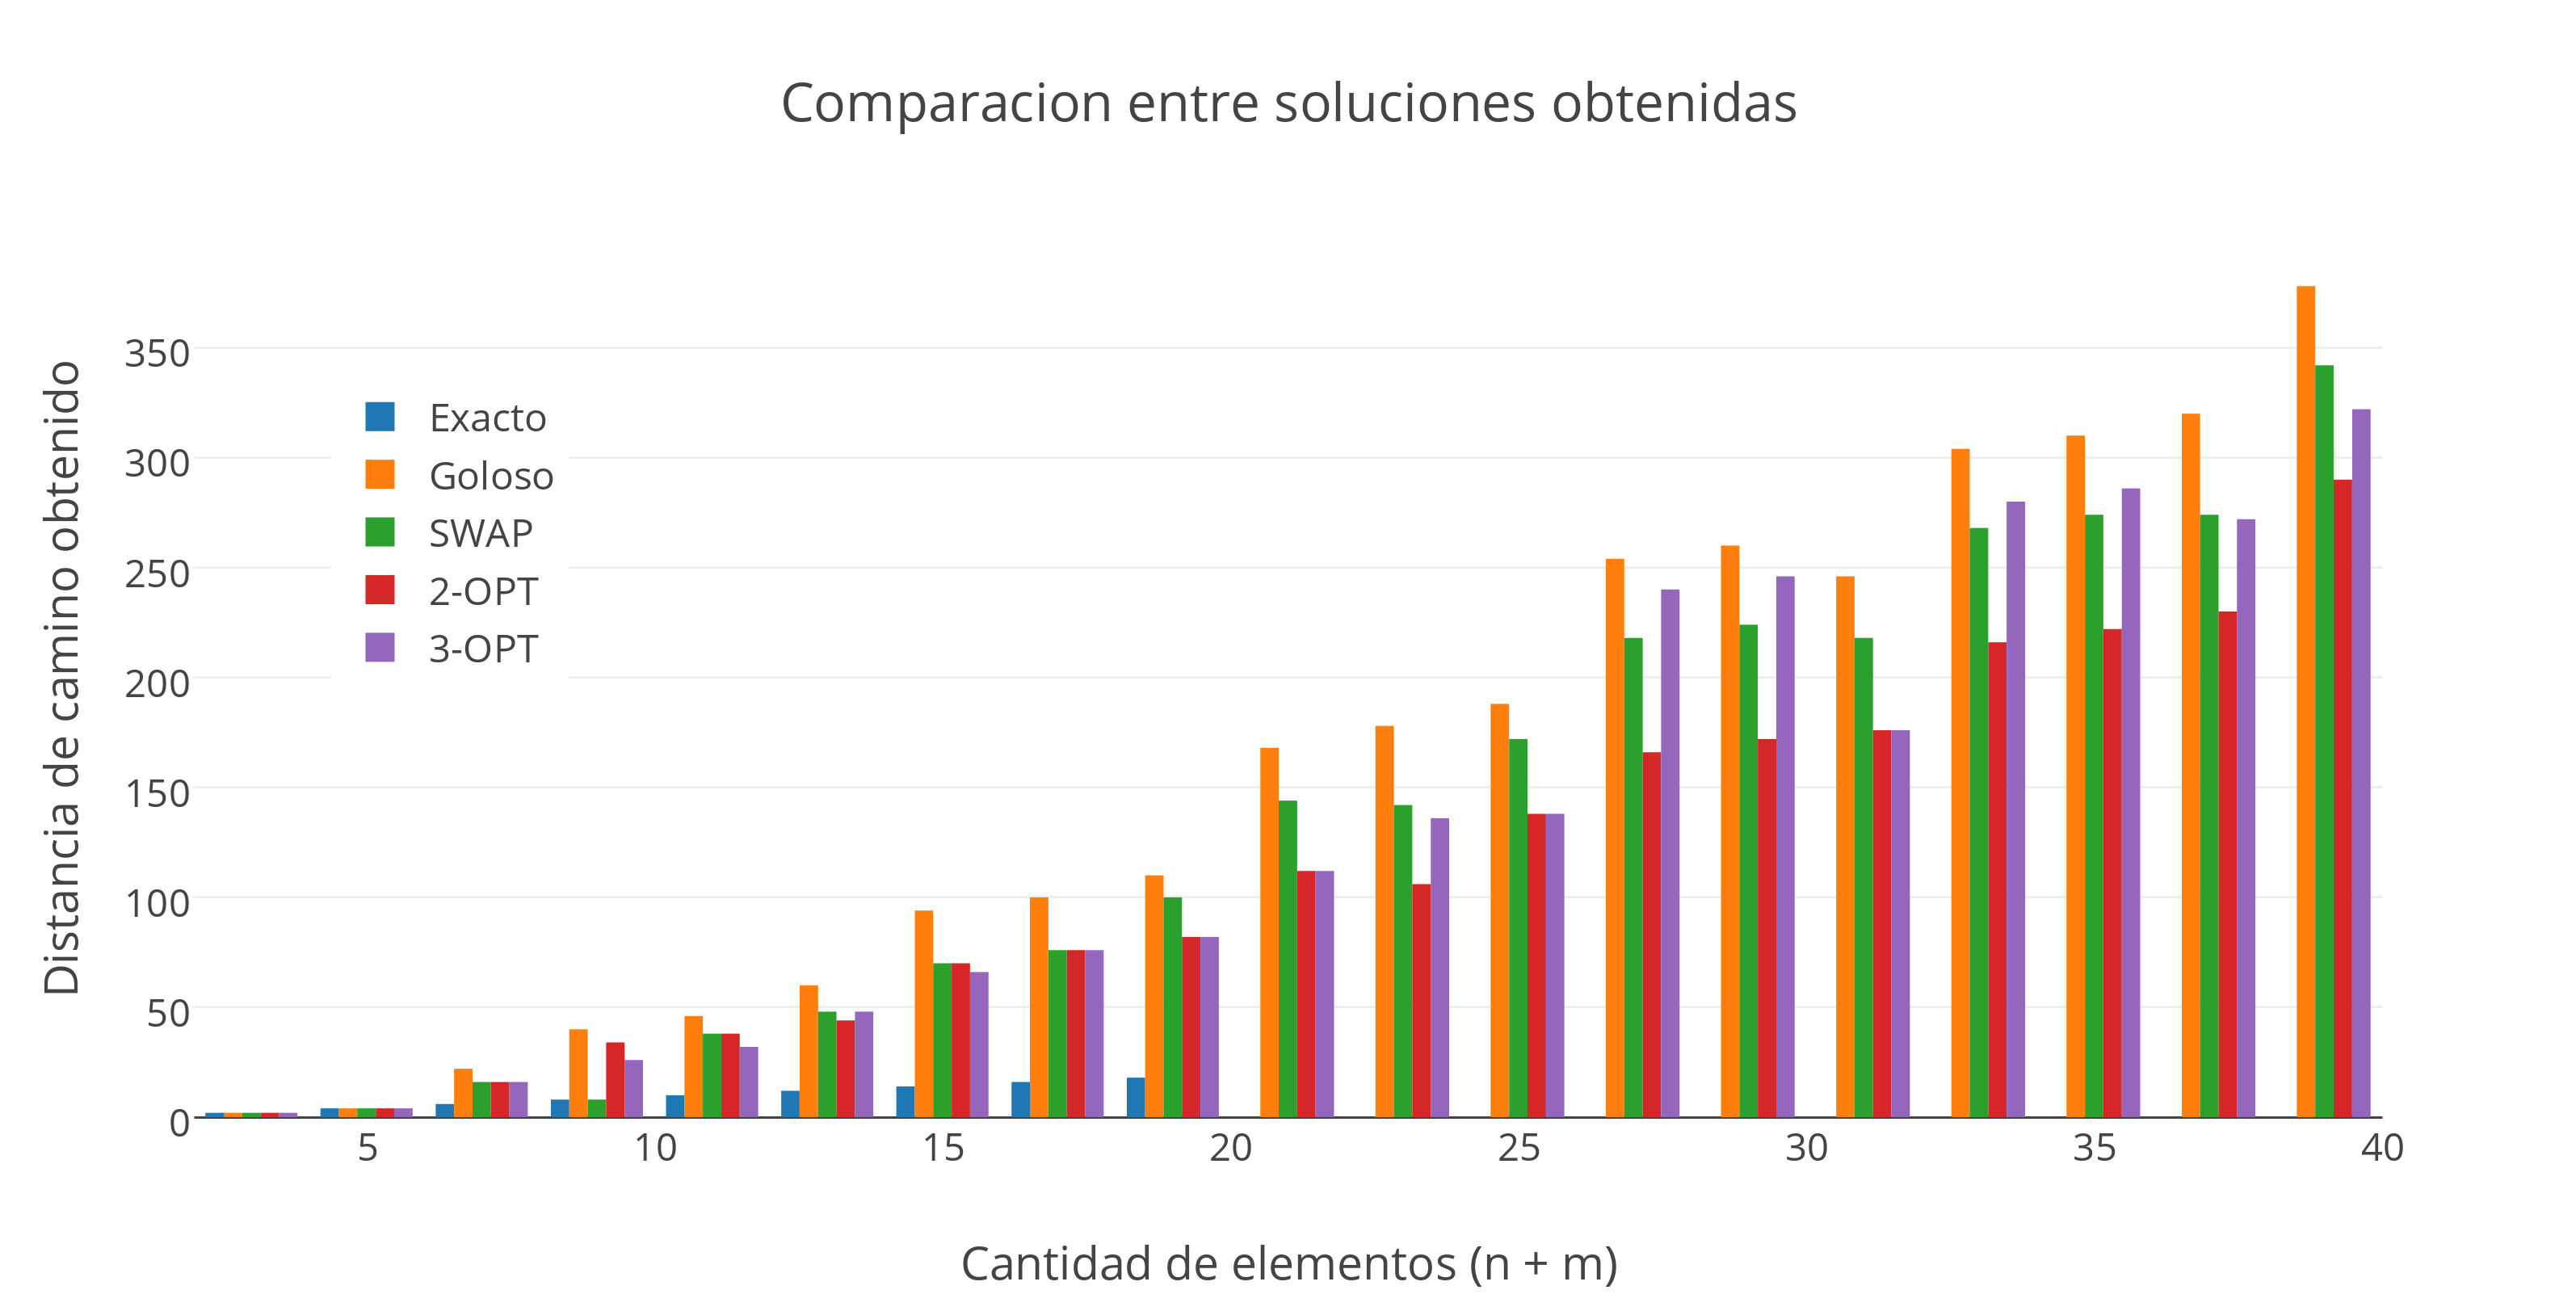
\includegraphics[scale=0.5]{./EJ3/comparacionbusquedaslocalessoluciongym0.png}
 {            \textit{Gráfico \ 3.1 - Búsquedas locales sobre Familia 4}}
  \end{center}
  \vspace*{0.3cm}
  
En cuanto a tiempo insumido vemos lo siguiente:

\vspace*{0.3cm} \vspace*{0.3cm}
  \begin{center}
 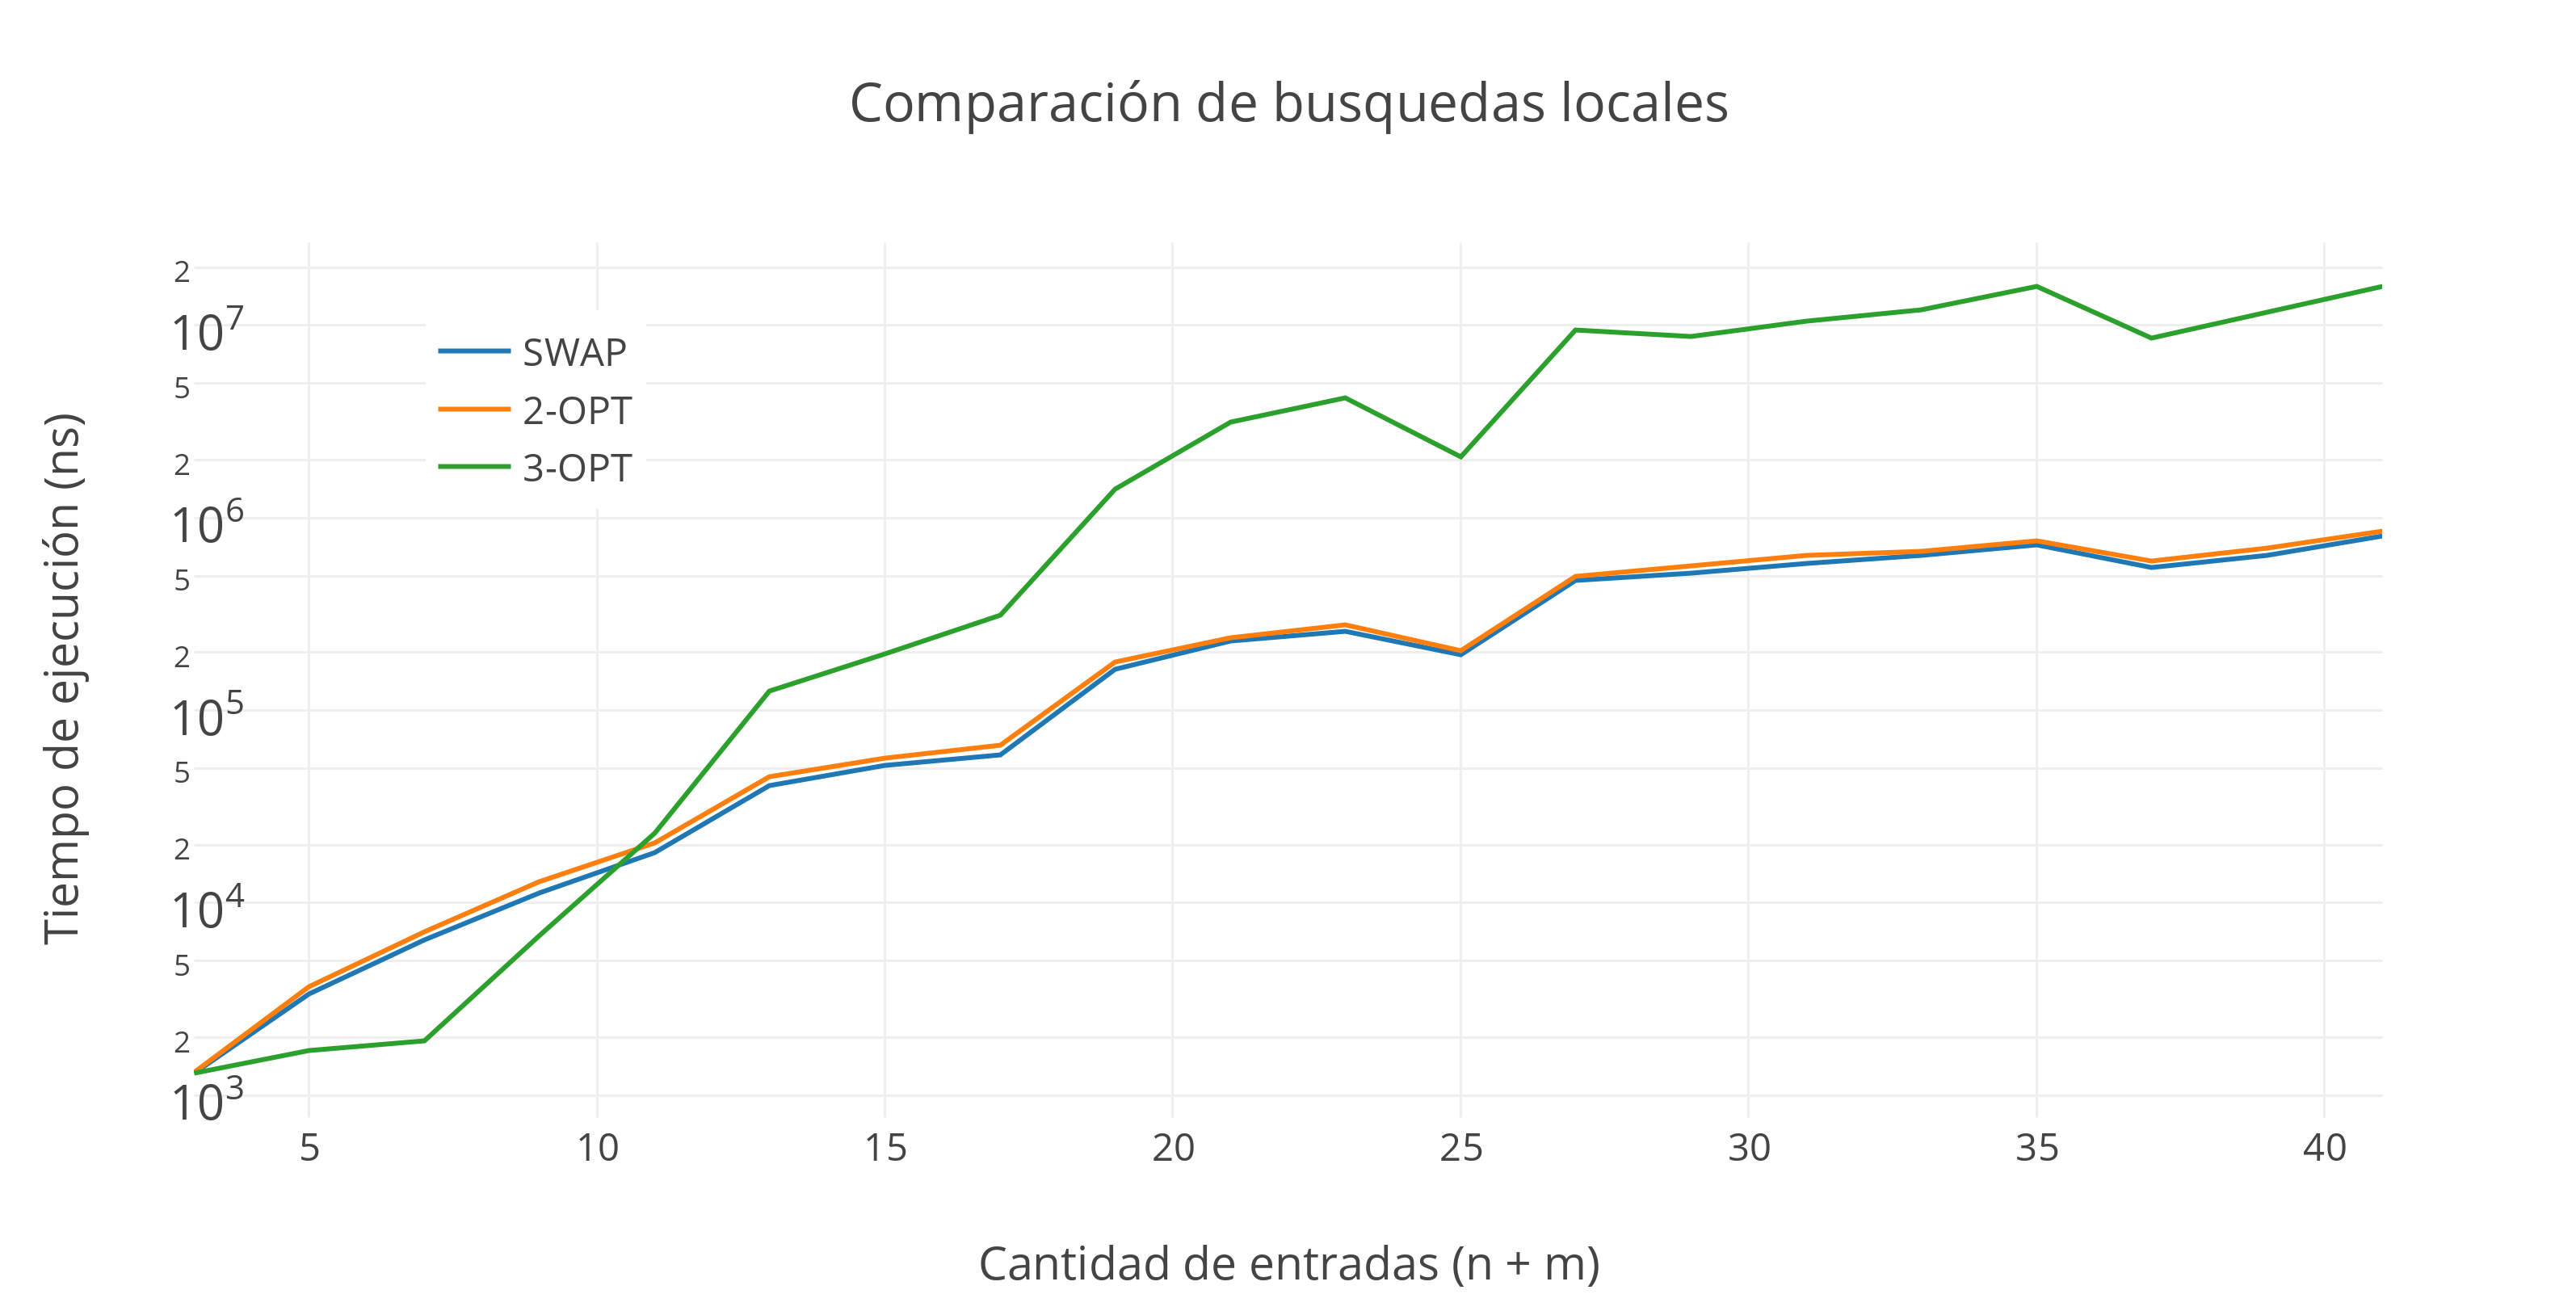
\includegraphics[scale=0.5]{./EJ3/comparacionbusquedaslocalesgym0.png}
 {            \textit{Gráfico \ 3.2 - Búsquedas locales sobre Familia 4}}
  \end{center}
  \vspace*{0.3cm}

  
 En este caso, el tiempo de ejecuci\'on de SWAP y 2-OPT tienen un desempeño temporal muy similar, no obstante, al comparar la calidad de solución, 2-OPT posee los mejores resultados. En cuanto a la variante 3-OPT: no solo genera peores soluciones, sino que tarda mucho más que las otras 2. 


\subsubsection*{Familia 6}


\vspace*{0.3cm} \vspace*{0.3cm}
  \begin{center}
 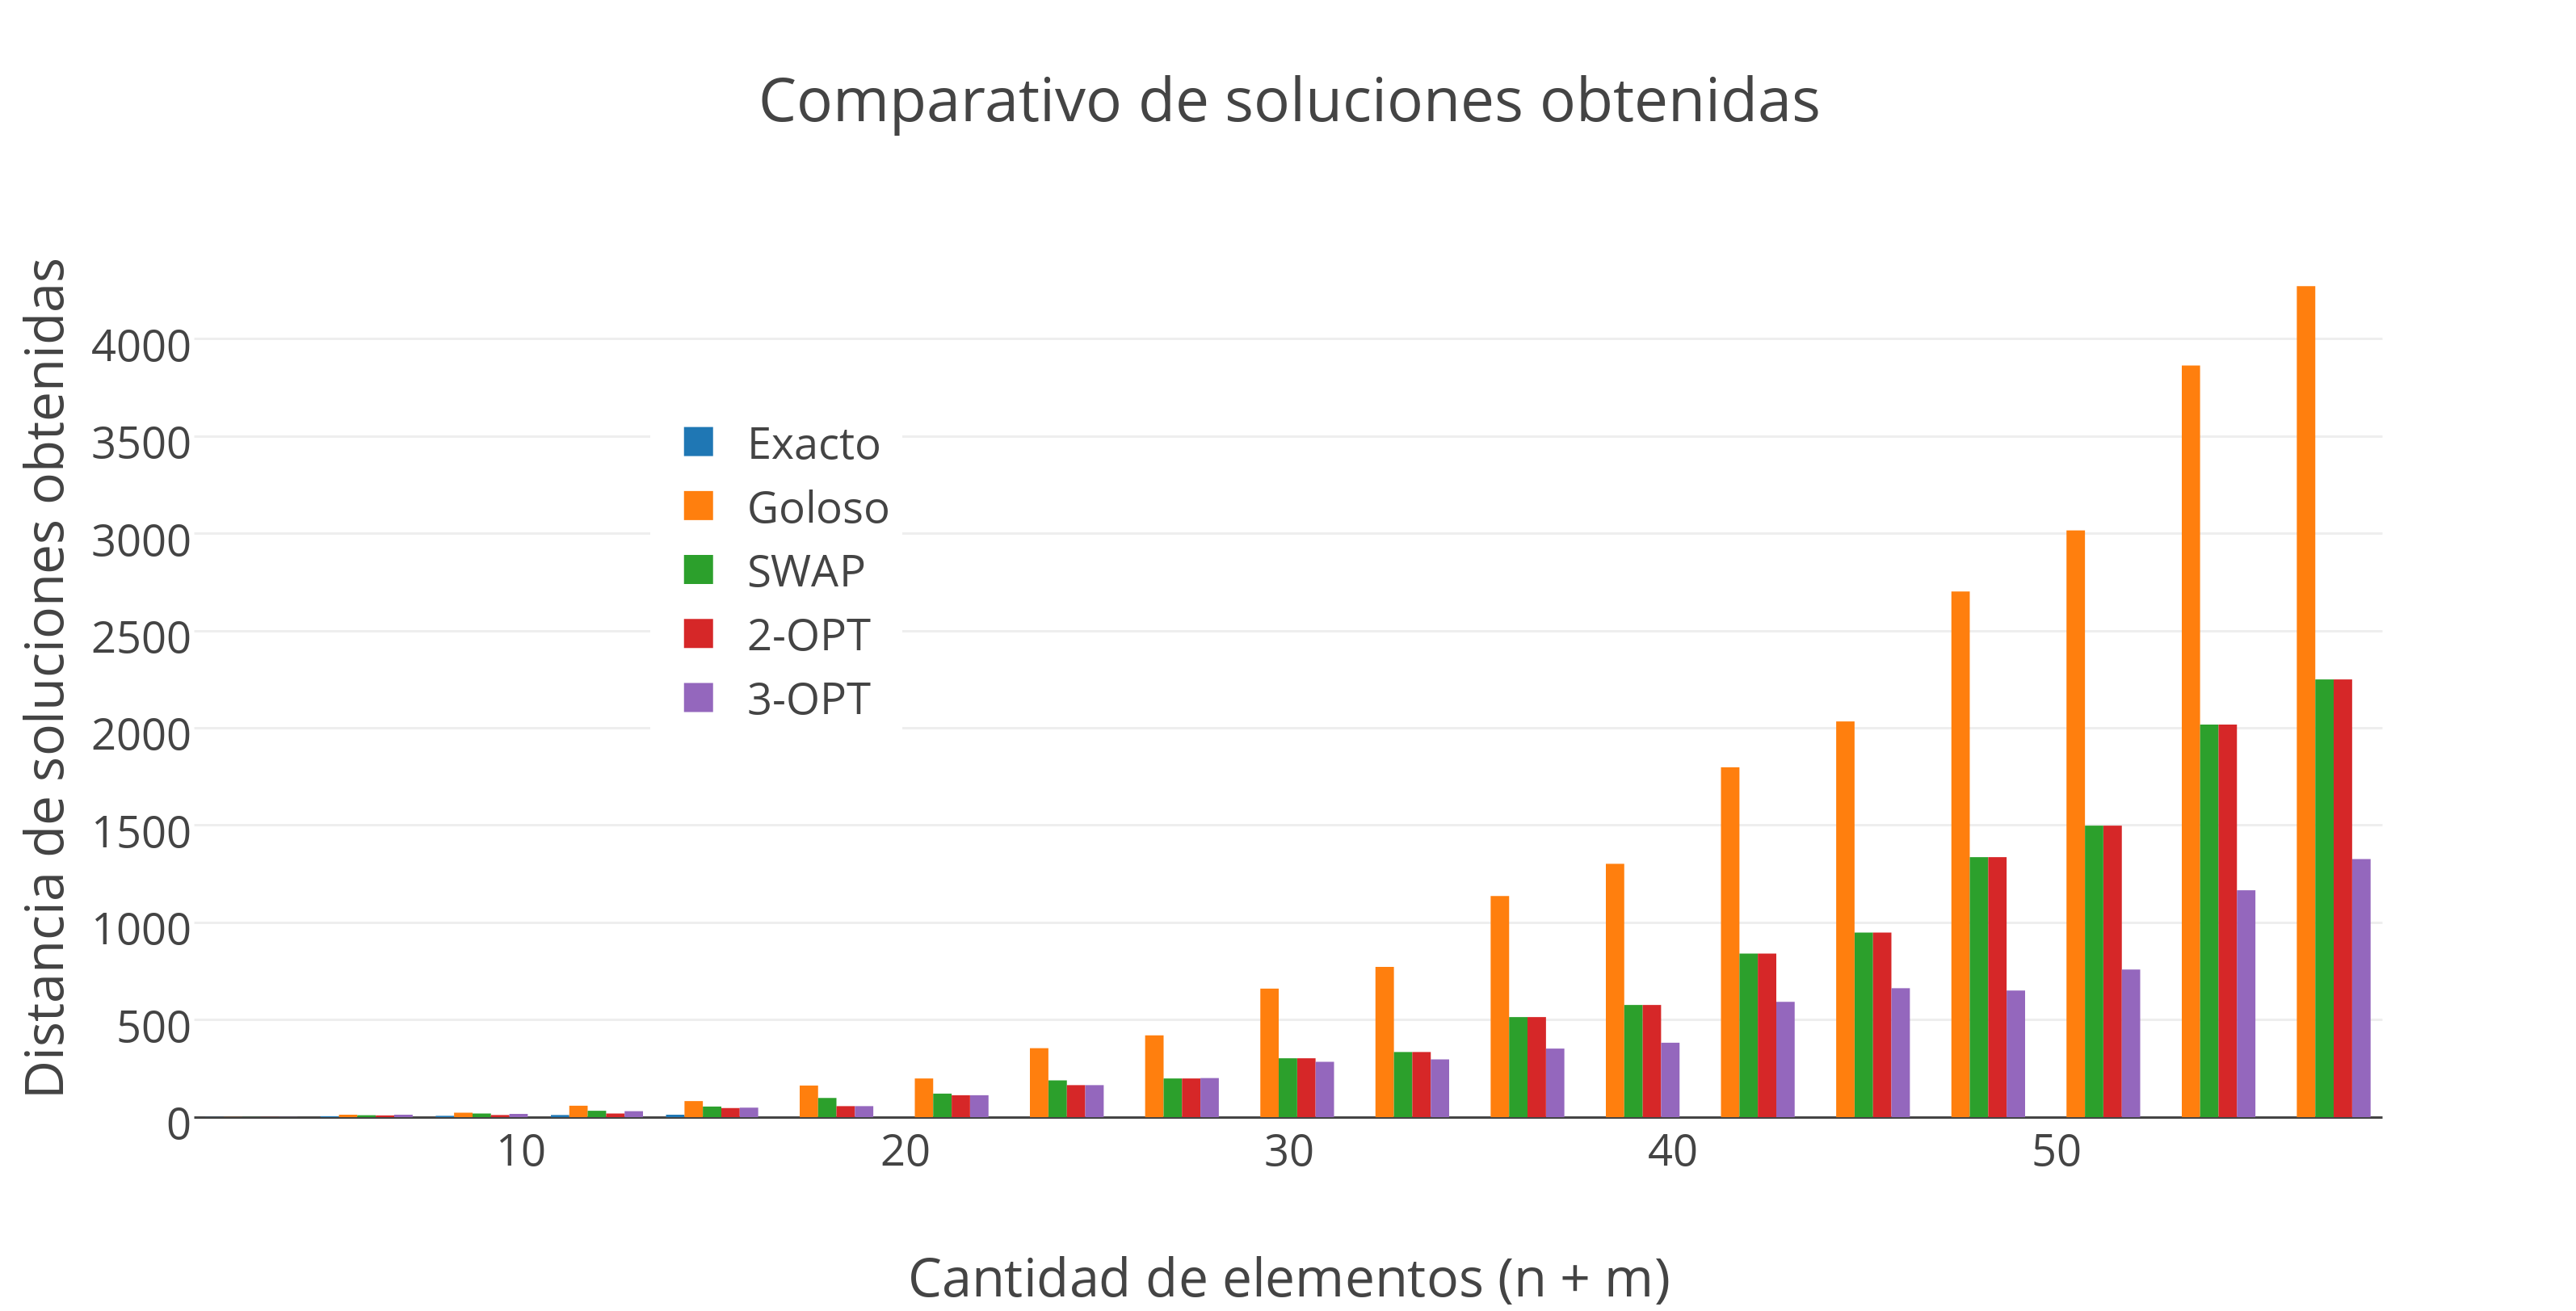
\includegraphics[scale=0.5]{./EJ3/comparacionbusquedaslocalessolucionsinorden.png}
 {            \textit{Gráfico \ 3.4 - Búsquedas locales sobre Familia 6}}
  \end{center}
  \vspace*{0.3cm}


\vspace*{0.3cm} \vspace*{0.3cm}
  \begin{center}
 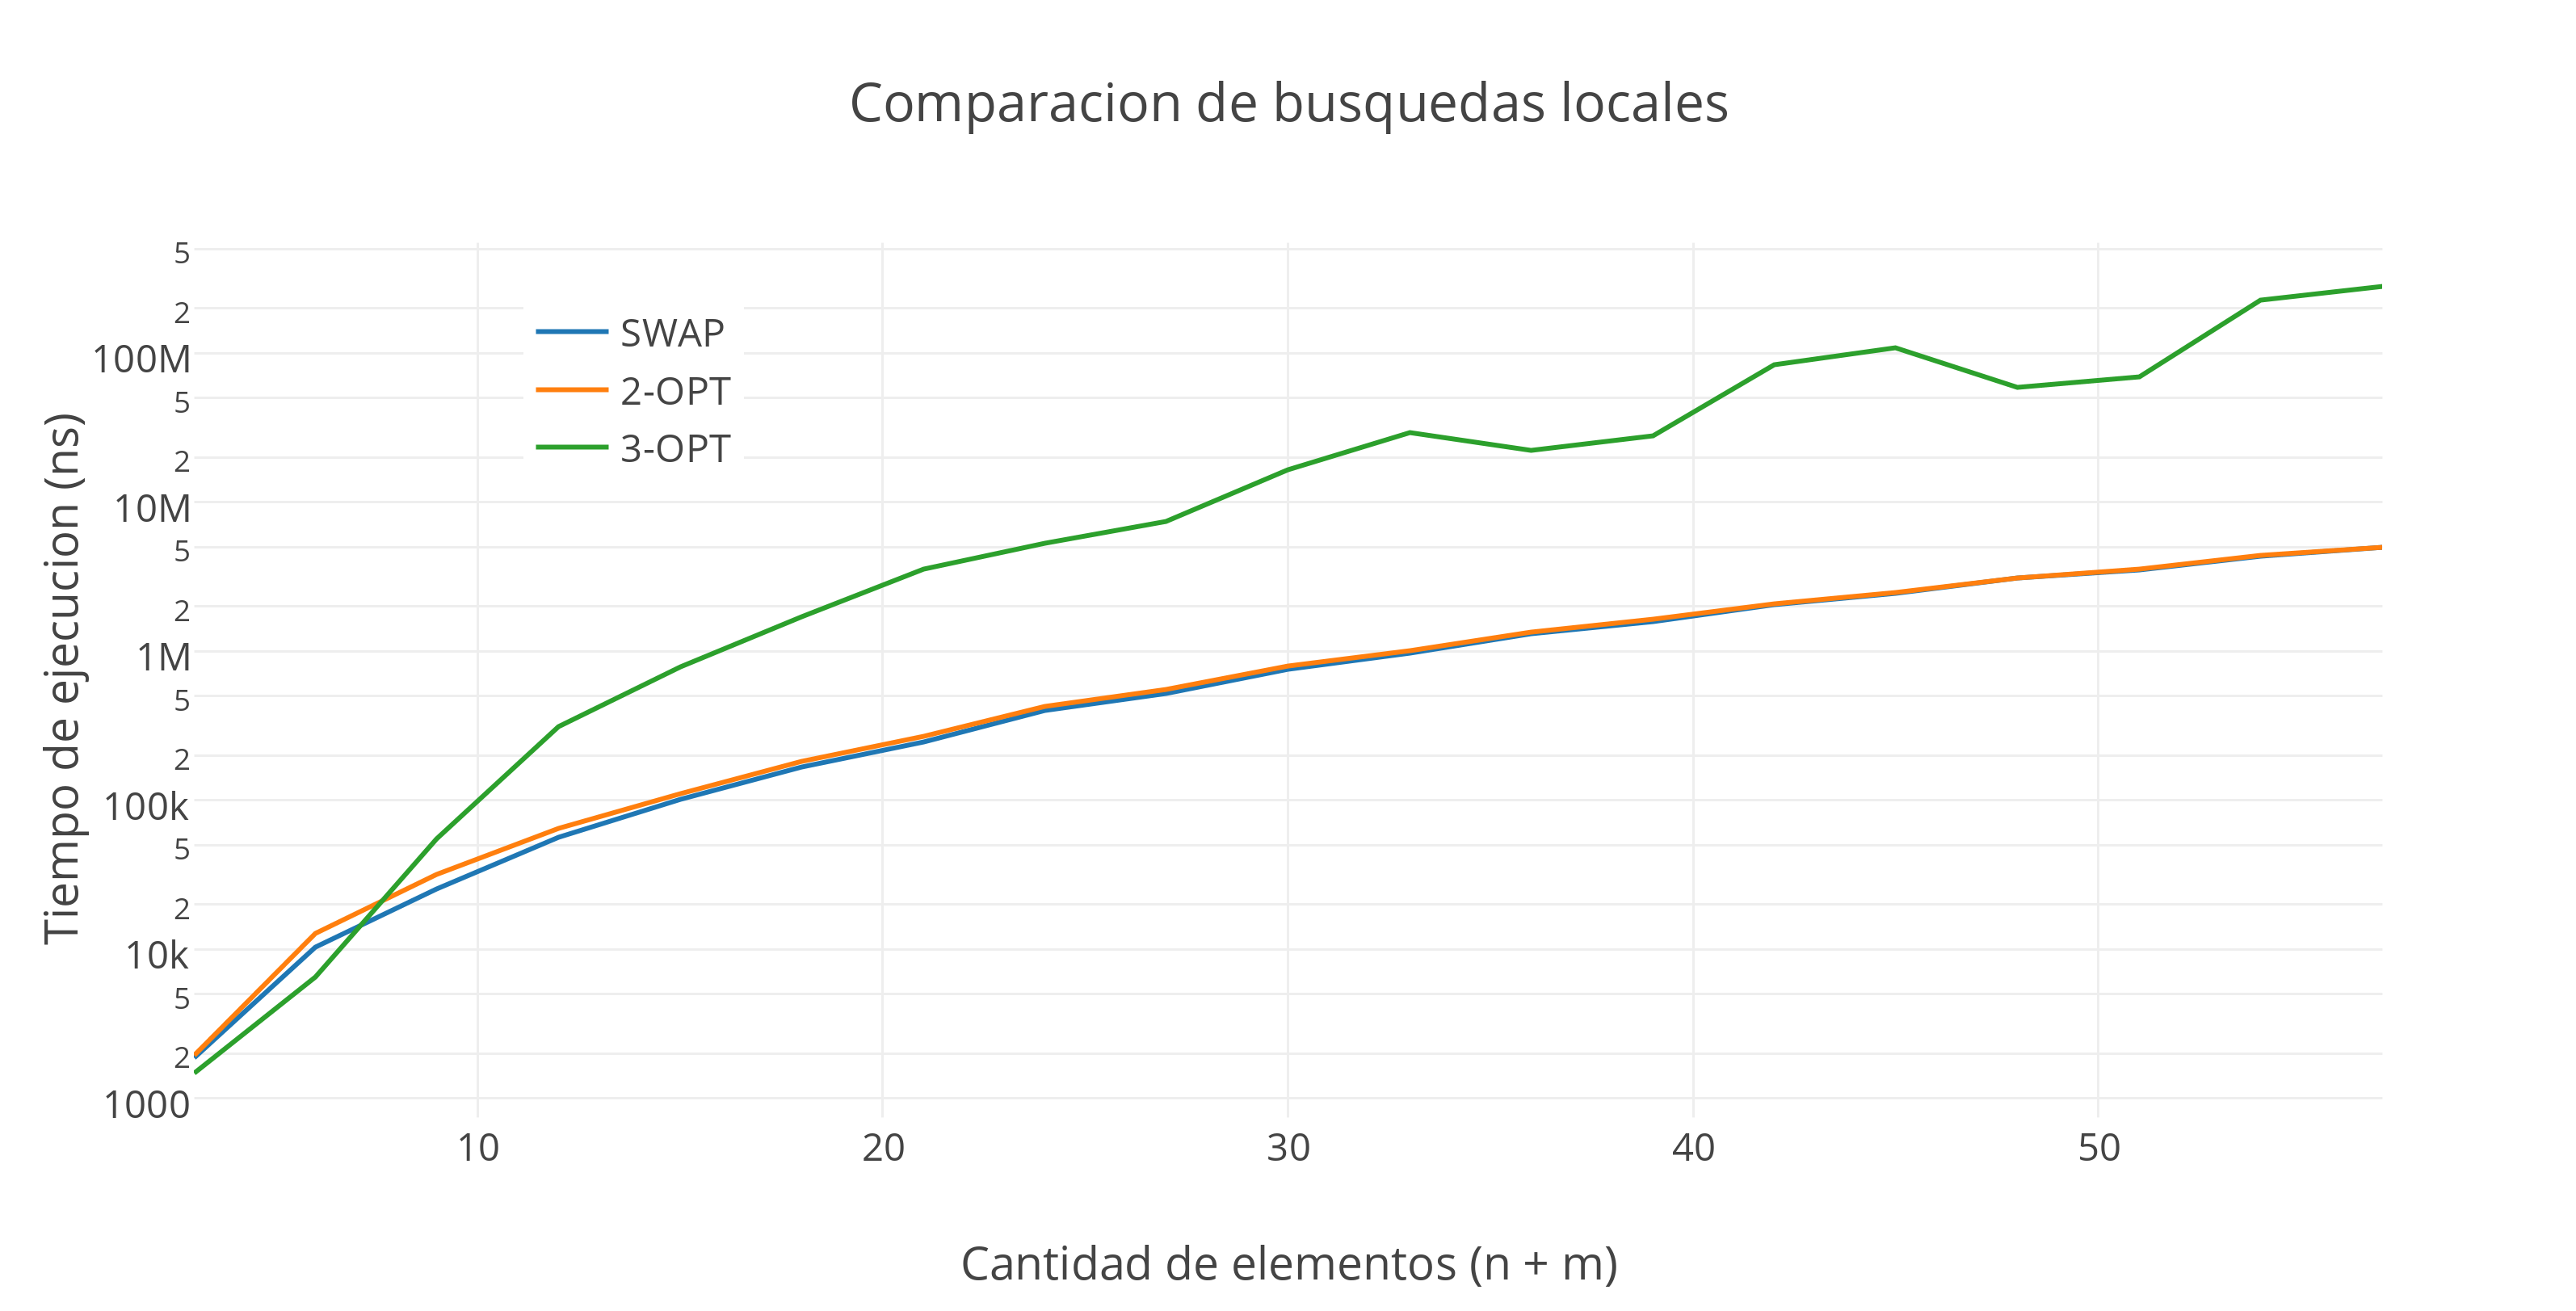
\includegraphics[scale=0.5]{./EJ3/comparacionbusquedaslocalessinorden.png}
 {            \textit{Gráfico \ 3.3 - Búsquedas locales sobre Familia 6}}
  \end{center}
  \vspace*{0.3cm}



Esta familia también muestra que a raz\'on de comparación en el tiempo de ejecución, SWAP es muy similar a 2-OPT y que 3-OPT posee el peor desempeño. Nuevamente podemos ver que a razón de calidad, 2-OPT logra una calidad superior a las otras búsquedas.



\subsubsection*{Familia 7}

  \vspace*{0.3cm} \vspace*{0.3cm}
  \begin{center}
 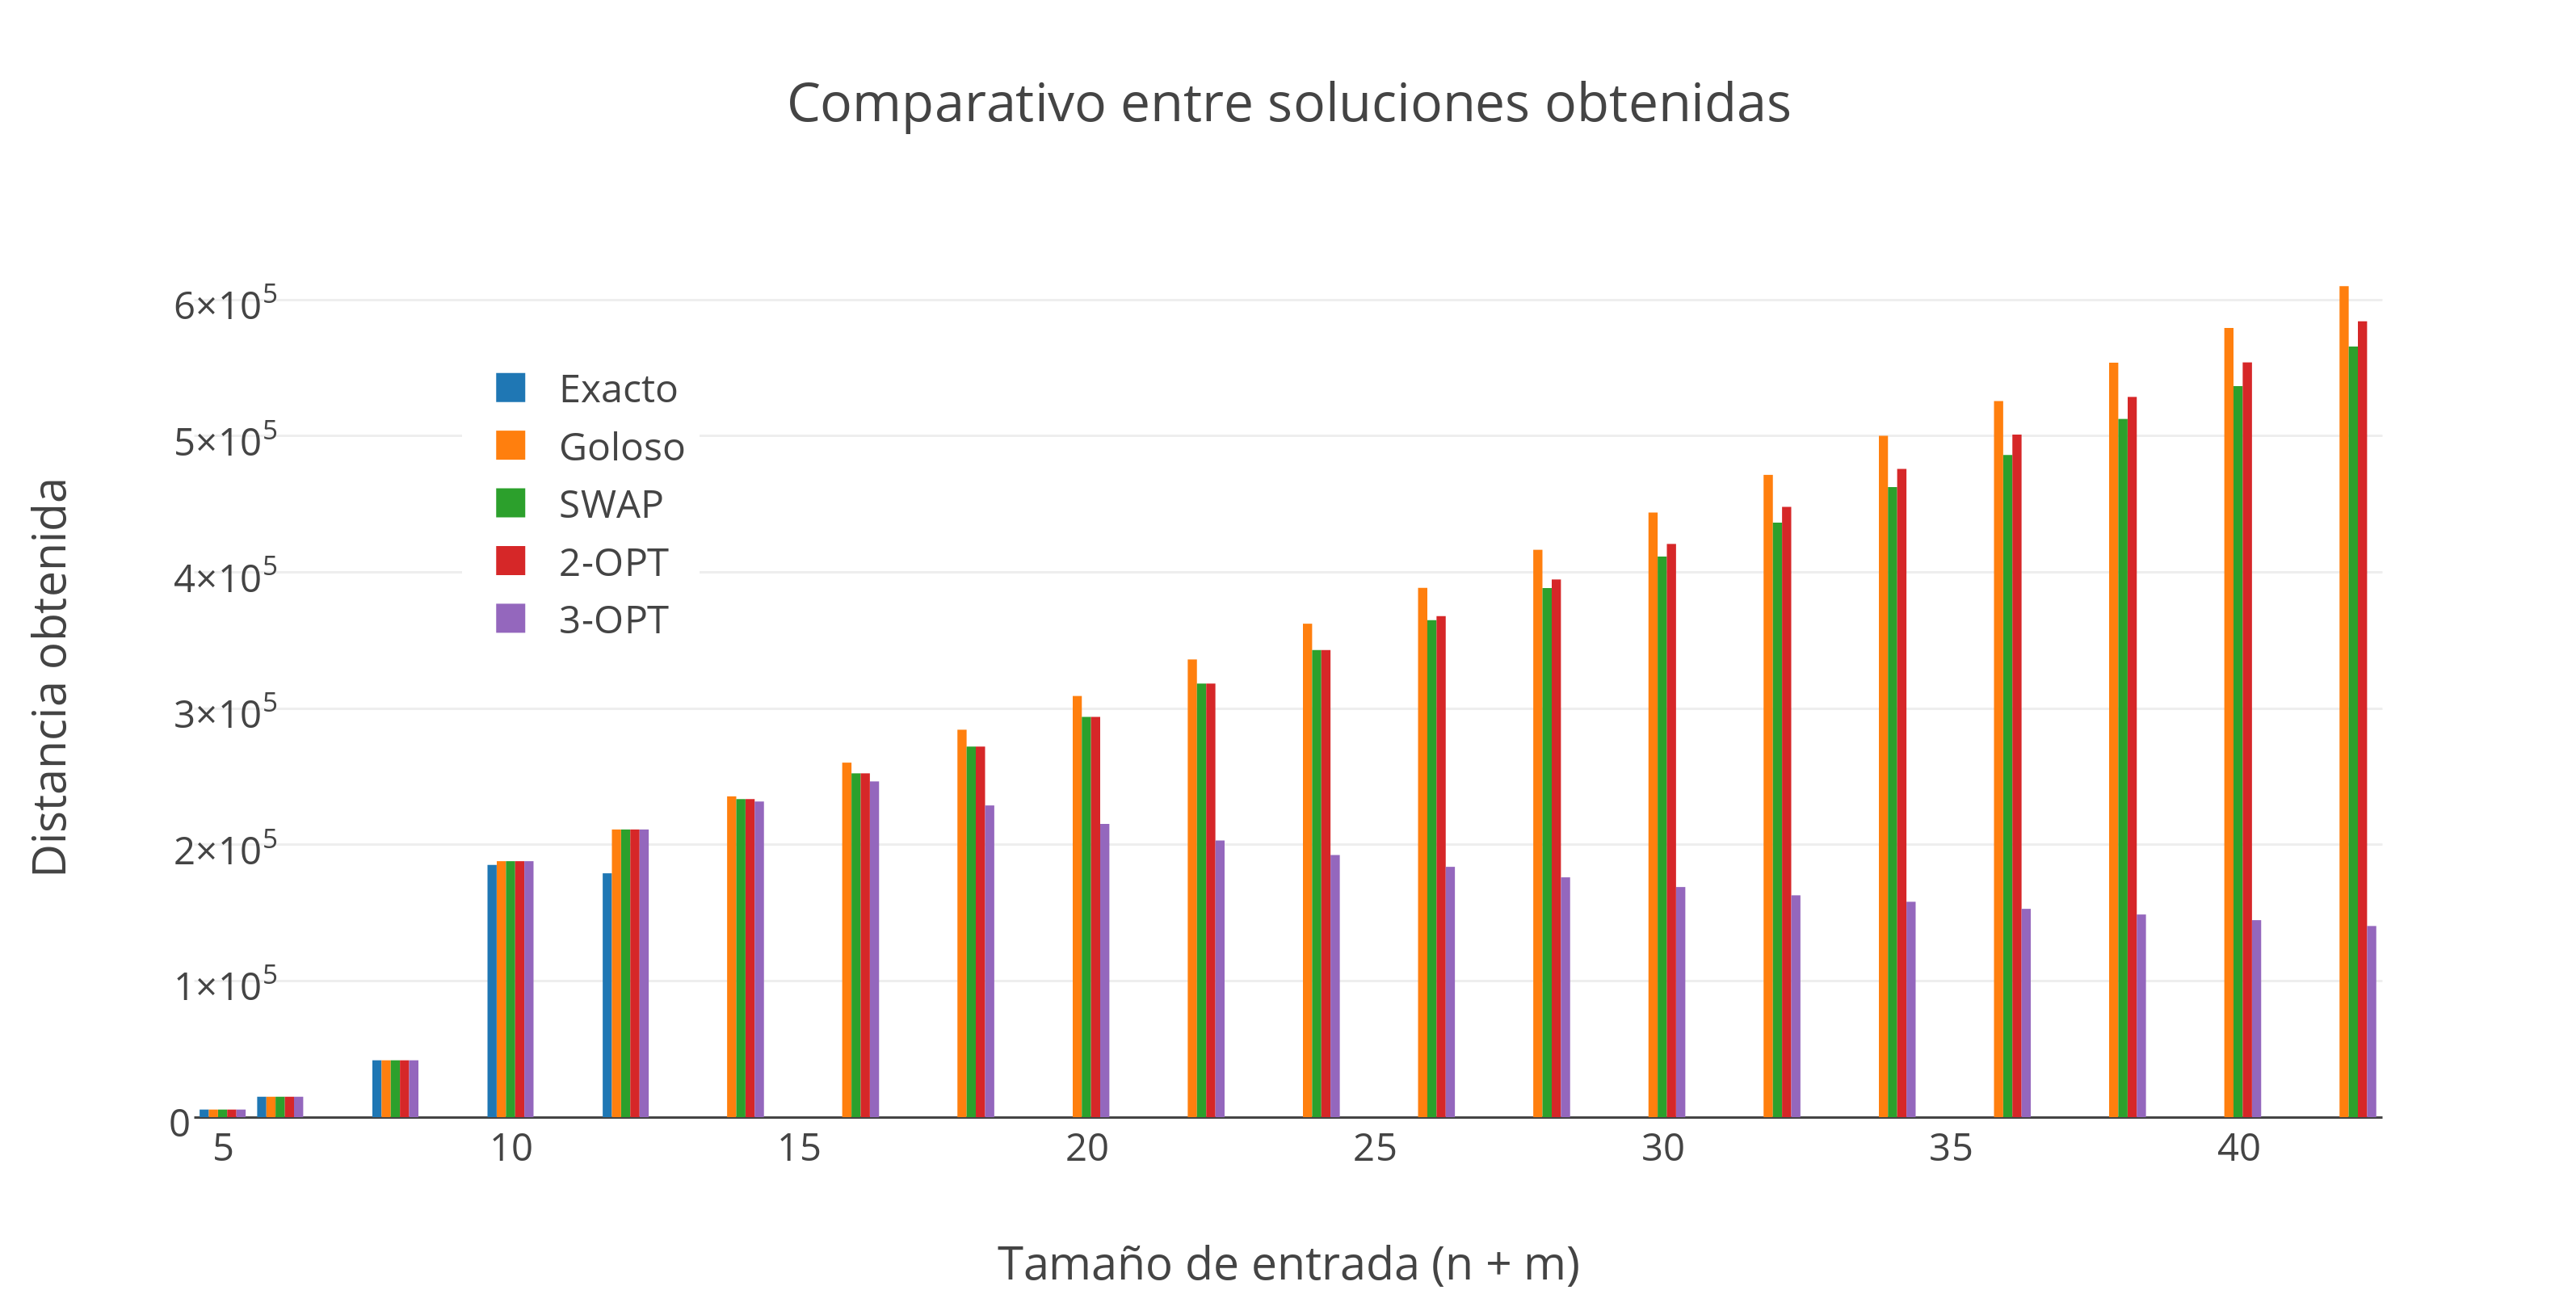
\includegraphics[scale=0.5]{./EJ3/comparacionbusquedaslocalessolucionanillos.png}
 {            \textit{Gráfico \ 3.6 - Búsquedas locales sobre Familia 7}}
  \end{center}
  \vspace*{0.3cm}

\vspace*{0.3cm} \vspace*{0.3cm}
  \begin{center}
 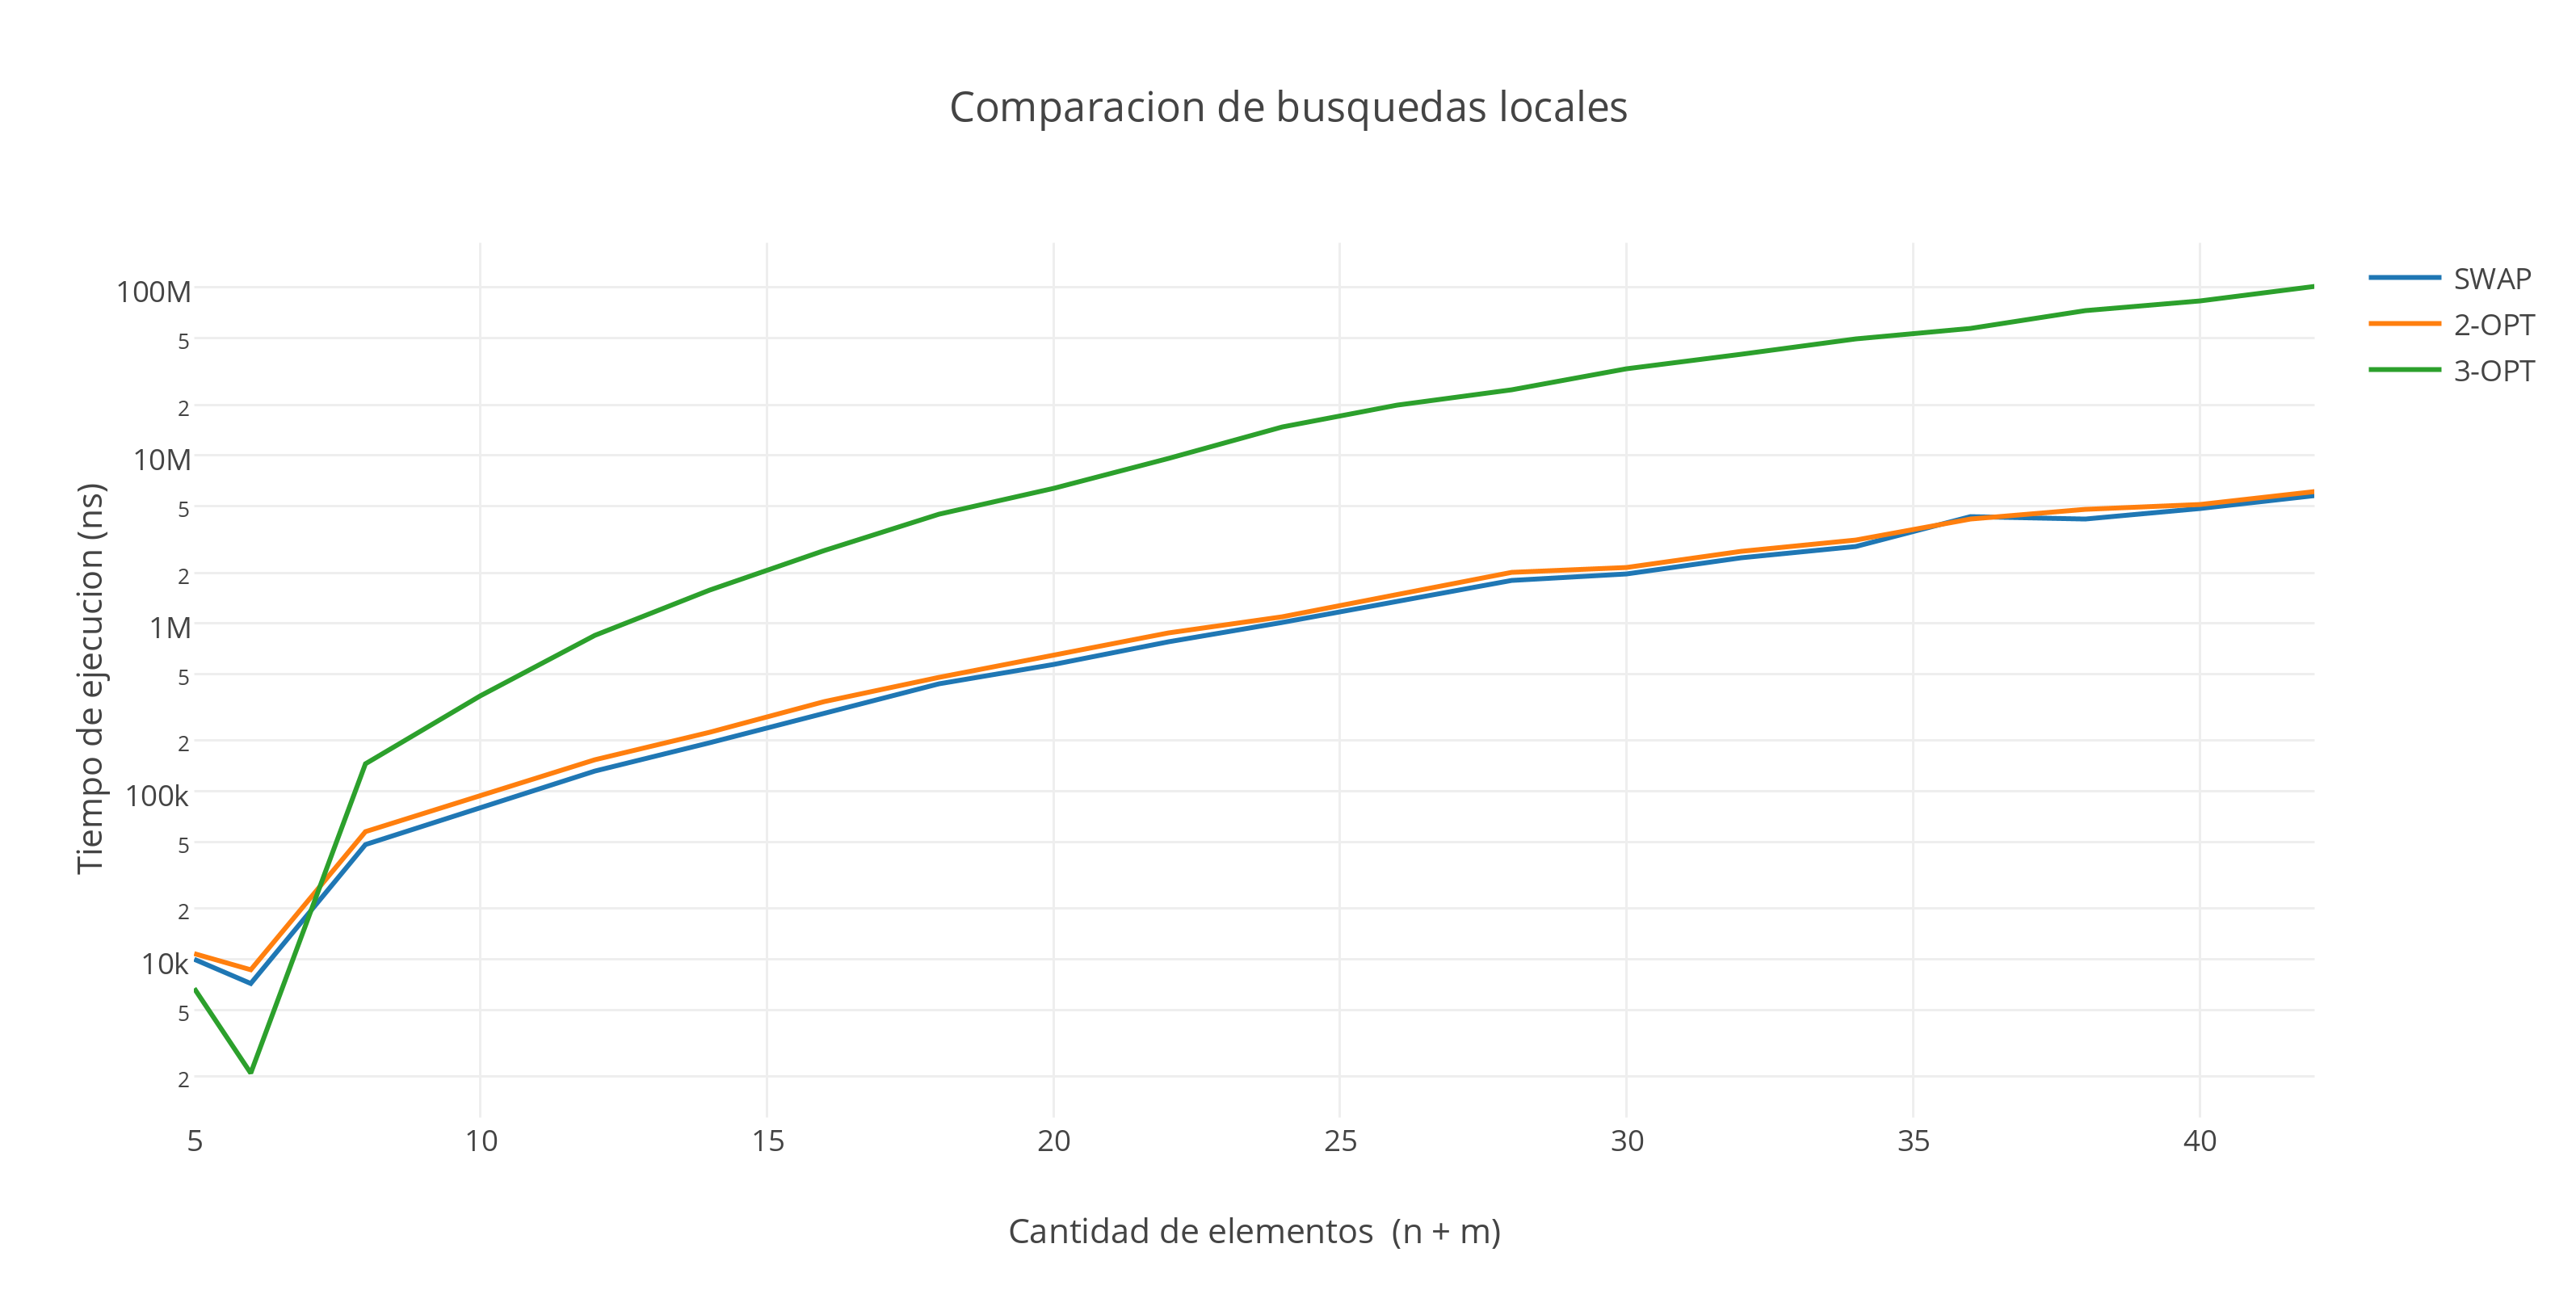
\includegraphics[scale=0.5]{./EJ3/comparacionbusquedaslocalesanillos.png}
 {            \textit{Gráfico \ 3.5 - Búsquedas locales sobre Familia 7}}
  \end{center}
  \vspace*{0.3cm}
  
  
  Los resultados se repiten como en las anteriores familias, marcando una clara diferencia temporal entre 3-OPT y las otras 2 busquedas. En cuanto a la calidad de soluci\'on, podemos ver que en este caso la heur\'istica 3-OPT logra una calidad superior que en las otras. Sin embargo, si se toma la relaci\'on tiempo-calidad la mejor opcion ser\'a 2-OPT.
  
  
\subsubsection*{Familia 8}

\vspace*{0.3cm} \vspace*{0.3cm}
  \begin{center}
 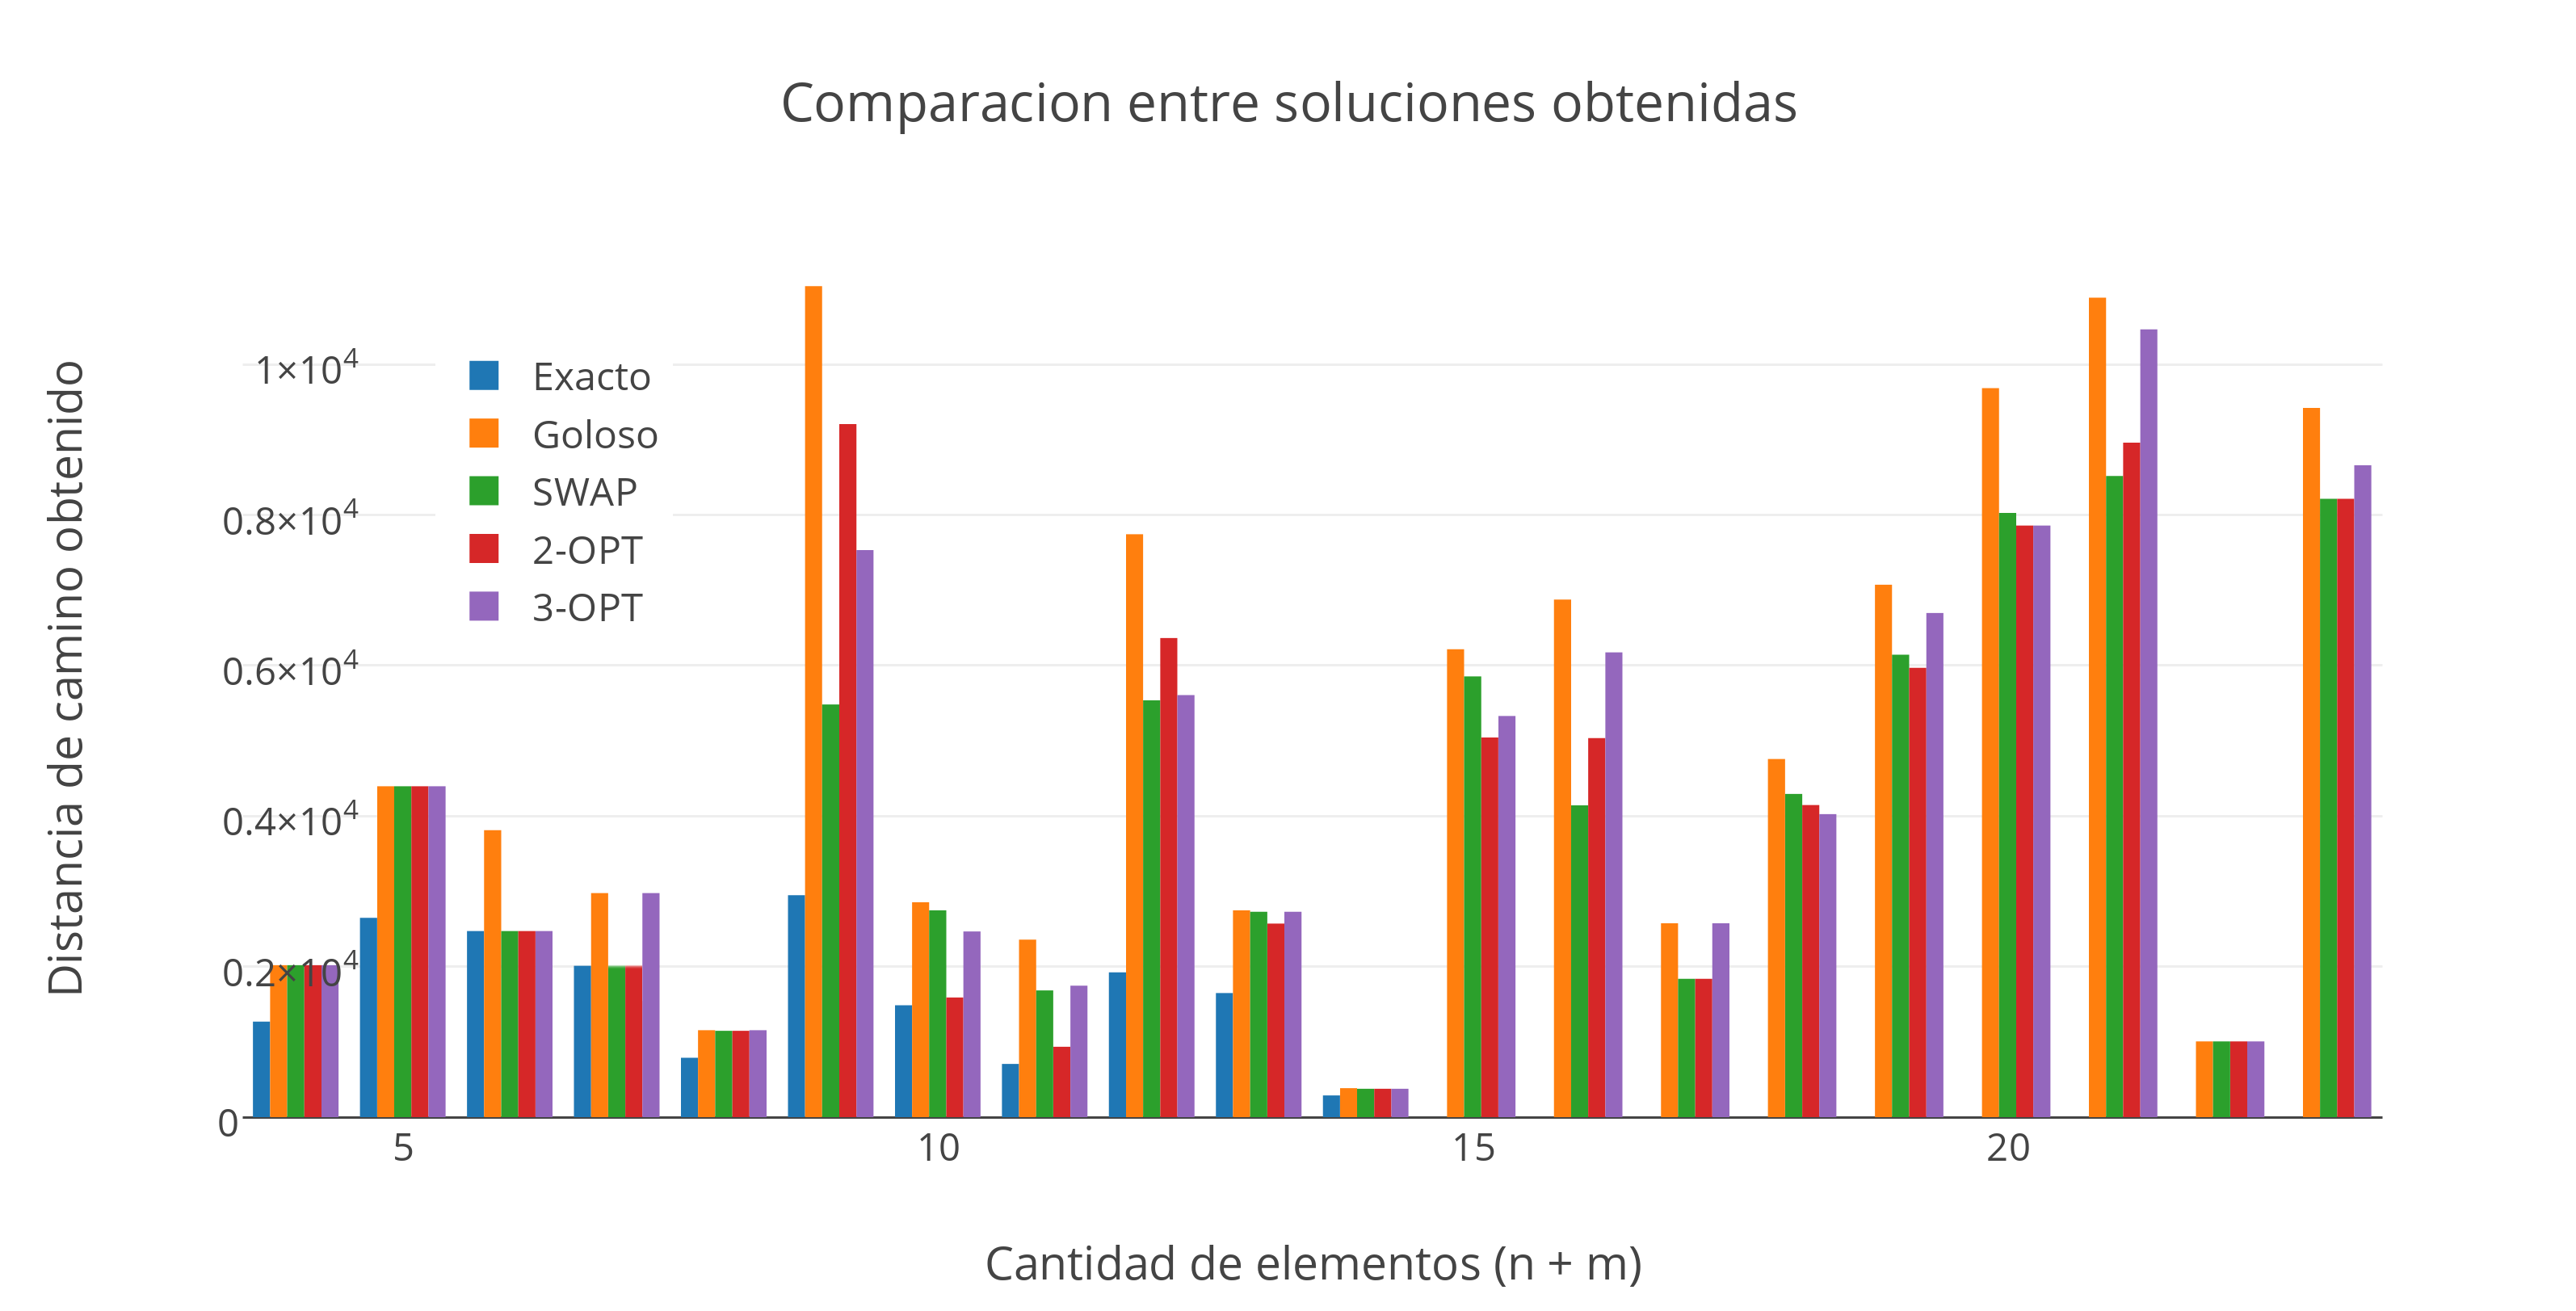
\includegraphics[scale=0.5]{./EJ3/comparacionbusquedaslocalessolucionrandom.png}
 {            \textit{Gráfico \ 3.7 - Búsquedas locales sobre Familia 8}}
  \end{center}
  \vspace*{0.3cm}
  

  Para este caso se evita la comparación de tiempo debido a que los resultados son equivalentes a los ya obtenidos, y no ofrecen información relevante.
  

Habiendo chequeado dichas mediciones de tiempo de los algoritmos, se pudo observar como 3-OPT presento una peor performance con las familias evaluadas. En relaci\'on a tiempo - calidad de soluci\'on el mejor termino siendo 2-OPT.